\documentclass[zihao=5, b5paper, twoside, heading=true, punct=kaiming]{ctexbook}
\usepackage[
  nomarginpar
  %, margin=.5in
  , top=1.5cm, bottom=1.5cm, left=2cm, right=2cm
]{geometry}

% ==================== Book flag==========================

\global\let\wholebook=\relax %without relax, we build article, esle book

\usepackage[cn]{prelude}

\setcounter{page}{1}

\graphicspath{
	{img/}
}

\makeindex

\begin{document}

% set PDF properties
\hypersetup{pdftitle={A tour of number},
            pdfauthor={liuxinyu99@hotmail.com},
            pdfsubject={Popular Science},
            pdfkeywords={Mathematics}}

% ================================================================
%                 COVER PAGE
% ================================================================

\title{
  {\bf \Huge 数的旅程}
  \centering
  \scalebox{0.4}{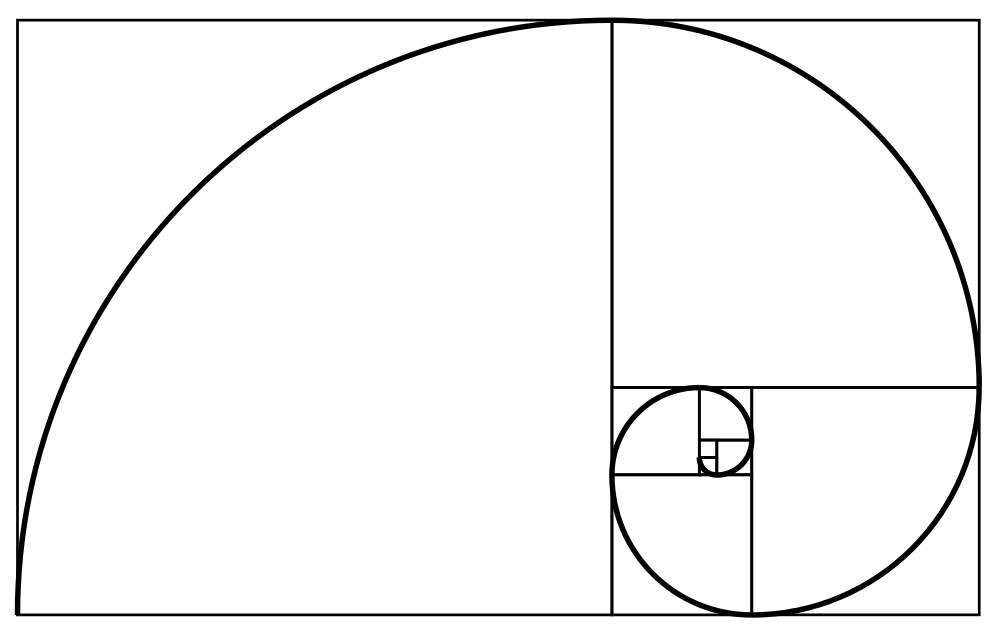
\includegraphics{img/fibonacci-spiral}}
}

\author{刘新宇
  \thanks{{\bfseries 刘新宇} \newline
    Version: $\displaystyle \phi = \frac{\sqrt{5} - 1}{2} = 0.618$ \newline
    \url{https://github.com/liuxinyu95} \newline
    }}

\maketitle

\frontmatter
%% \subimport{path/}{preface-zh-cn.tex}
\newpage

\tableofcontents

\mainmatter

%% \subimport{path/}{ancient-zh-cn.tex}

\appendix

%% \subimport{path/}{appendix-zh-cn.tex}

\chapter{参考答案}
\label[appendix]{ch:answers}
\phantomsection
\shipoutAnswer

%% \subimport{path-to-appendix/}{bib-zh-cn.tex}

\backmatter
\phantomsection
\addcontentsline{toc}{chapter}{\indexname}
\printindex

%% \subimport{}{fdl-1.3.tex}
\end{document}
